\chapter{Estratégia de Go com Compensação}\label{chap:estrat_comp}

Depois de ter estudado, nos capítulos anteriores deste livro, e jogado algumas partidas em tabuleiros menores, você já adquiriu um conhecimento básico das regras e táticas básicas, então já está bem encaminhado para se tornar um jogador de Go. O próximo tópico que você precisará aprender é o de princípios básicos de estratégia do jogo. A forma mais segura de aprender tais princípios é estudando Go com pedras de compensação. Isso significa procurar por oponentes mais fortes e, com prazer, tomar grandes compensações contra eles. Jogar Go com compensação vai lhe ensinar como utilizar suas pedras de vantagem para ganhar influência no centro. Apesar de que o objetivo do Go é assegurar mais território do que o adversário, é influência que, lenta mas certamente, se torna (mais) território.

A maior compensação que existe tradicionalmente é a de nove pedras. É na verdade uma compensação enorme, equivalente a uma rainha no xadrez, ou talvez mais. Ainda assim, como iniciante, levará um bom tempo antes que você possa derrotar até mesmo um 1 dan razoavelmente forte, com essa compensação.

Encontrar oponentes hoje em dia é fácil. Há um excelente servidor chamado KGS (\href{https://www.gokgs.com}{\path{gokgs.com}})~\cite{kgs} onde você pode jogar online gratuitamente e, ainda, encontrar adversários desde a sua própria força até a de profissionais.

Como introdução, nós restringiremos esta discussão à compensação de nove pedras e somente estudaremos alguns padrões básicos que surgem com frequência neste nível de compensação.

\pagebreak

\begin{wrapfigure}{r}{60mm}
    \vspace{-15pt}
    \begin{center}
        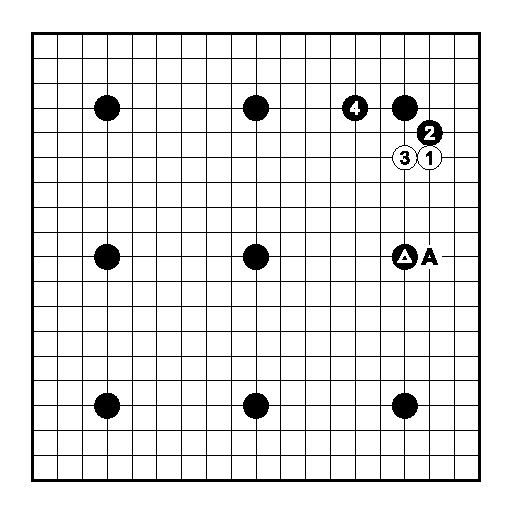
\includegraphics[width=.5\textwidth]{9 - Dia 1}
        \captionsetup{justification=centering}
        \caption*{\emph{Dia.\@~1}}
    \end{center}
    \vspace{-20pt}
\end{wrapfigure}

Branco geralmente começa se aproximando de uma das pedras de compensação no canto com 1 no \emph{Dia.\@~1}. A resposta preta mais forte é contatar com o movimento diagonal de 2. Branco responde, na maioria das vezes, estendendo em 3, e Preto pode delimitar seu território no topo com 4.

A razão pela qual a troca de Preto 2 por Branco 3 é boa para Preto é que a pedra marcada está atacando as duas pedras brancas. Em outras palavras, ela está atuando como uma pinça em conjuntura com as três pedras pretas no topo.

Idealmente, Branco gostaria de estender tão longe quanto \textbf{A}, mas a pedra marcada está no caminho. (Vide os princípios de extensão discutidos na seção \autoref{sec:6.6:extensions}.)

\begin{wrapfigure}{l}{60mm}
    \vspace{-25pt}
    \begin{center}
        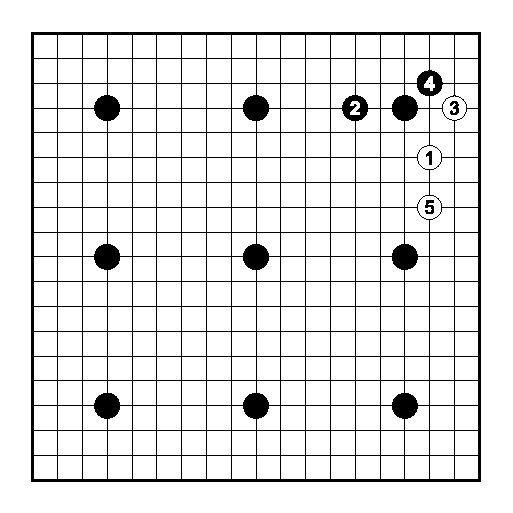
\includegraphics[width=.5\textwidth]{9 - Dia 2}
        \captionsetup{justification=centering}
        \caption*{\emph{Dia.\@~2}}
    \end{center}
    \vspace{-30pt}
\end{wrapfigure}

Para compreender a razão que faz com que Preto primeiro contate em 2, suponhamos que Preto omita tal jogada e simplesmente estenda para 2 no \emph{Dia.\@~2}. Branco poderia, então, deslizar a 3, Preto defende com a diagonal de 4, e Branco estende para 5. Comparado à posição em \emph{Dia.\@~1}, as pedras brancas terminam por ficar muito mais resilientes. Elas estão tomando território e estão muito mais avançadas no critério de fazer dois olhos e viver.

\pagebreak

\section{A Estratégia Branca de Chapelação}

\begin{wrapfigure}{r}{60mm}
    \vspace{-27.5pt}
    \begin{center}
        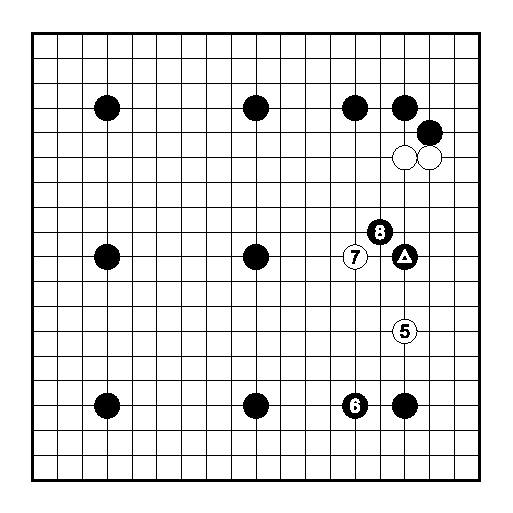
\includegraphics[width=.5\textwidth]{9 - Dia 3}
        \captionsetup{justification=centering}
        \caption*{\emph{Dia.\@~3}}
    \end{center}
    \vspace{-30pt}
\end{wrapfigure}

Após Preto 4 no \emph{Dia.\@~1}, Branco talvez faça a aproximação de dois espaços contra a pedra preta no canto inferior direito com 5 no \emph{Dia.\@~3}. Preto 6, delimitando o território no lado inferior, é um bom movimento e a resposta padrão. Branco poderá talvez, então, chapelar a pedra preta no lado direito com 7, ameaçando ostensivamente fazer território ele mesmo. Na realidade, ele está na esperança de atiçar Preto para uma briga, em que a habilidade de luta branca, sendo este o jogador mais forte, será muito superior à preta.

Como Preto deveria responder?

A melhor estratégia é resolutamente escapar ao centro com a pedra marcada, jogando a diagonal de 8.

\begin{wrapfigure}{l}{60mm}
    \vspace{-22.5pt}
    \begin{center}
        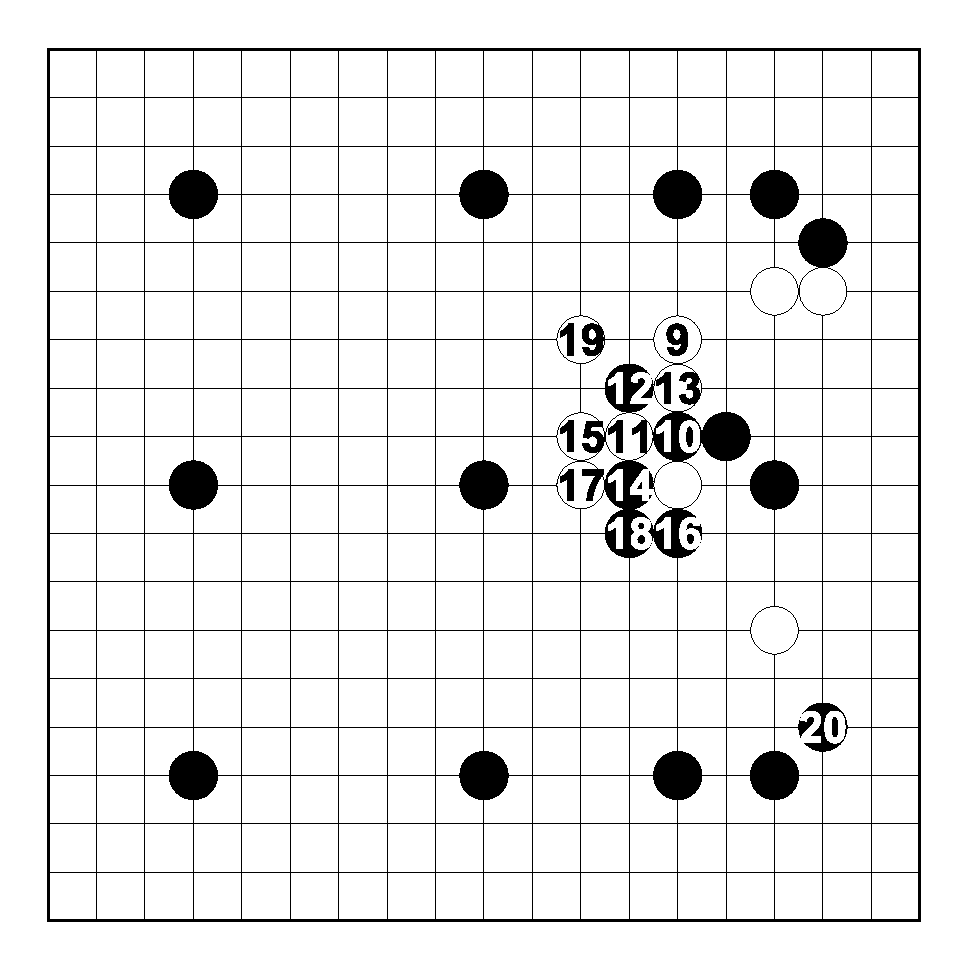
\includegraphics[width=.5\textwidth]{9 - Dia 4}
        \captionsetup{justification=centering}
        \caption*{\emph{Dia.\@~4}}
    \end{center}
    \vspace{-20pt}
\end{wrapfigure}

Branco tenta manter Preto confinado ao lado direito com 9 a 11 no \emph{Dia.\@~4}, mas, depois de 12, Branco precisa cortar em 13 para eliminar a conexão preta ali. Preto então faz atari com 14 a 16, e suas pedras agora escaparam. Branco faz atari com 17, e assegura sua posição com 19 --- Branco talvez também jogue em \textbf{A}. Após 20, Preto já quase assegurou a maior parte do território na parte baixa do lado direito. Exceto pela captura de 12, Branco não possui nenhum território.

\pagebreak

\begin{wrapfigure}{r}{60mm}
    \vspace{-17.5pt}
    \begin{center}
        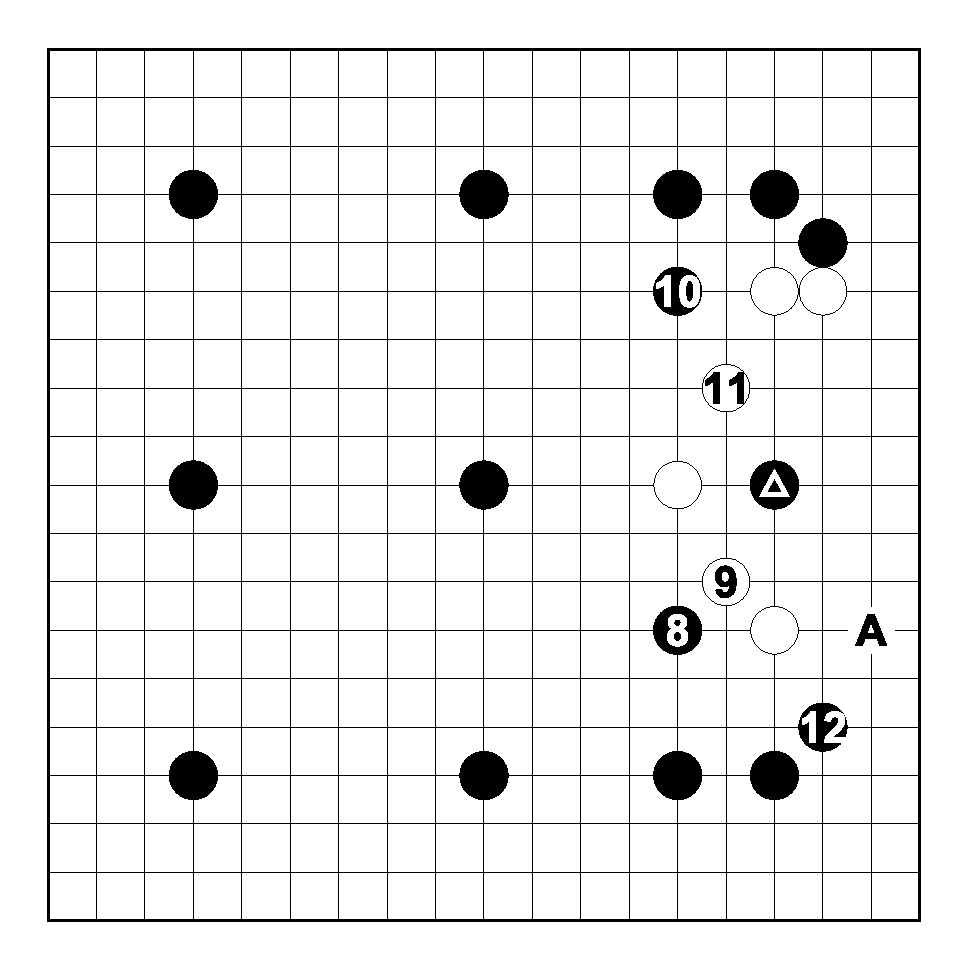
\includegraphics[width=.5\textwidth]{9 - Dia 5}
        \captionsetup{justification=centering}
        \caption*{\emph{Dia.\@~5}}
    \end{center}
    \vspace{-37.5pt}
\end{wrapfigure}

Outra estratégia que Preto pode empregar contra a estratégia branca de chapelação é a de ceder território no lado direito. Por exemplo, Preto pode começar por contra-chapelar em 8 no \emph{Dia.\@~5}, ameaçando se conectar com a pedra marcada. Branco defende em 9. Preto agora pula a 10, induzindo Branco a defender em 11. Preto agora expande seu território no canto com 12, ameaçando reduzir o território e expandir o seu ainda mais, através do deslize em \textbf{A}.

Branco provavelmente defenderá com 13 no \emph{Dia.\@~6}. Preto continuará ameaçando reduzir o território branco com 14 a 16, enquanto expande seus cantos direitos superior e inferior. A continuação até 25 ainda também termina em sente.

\begin{wrapfigure}{l}{60mm}
    \vspace{-22.5pt}
    \begin{center}
        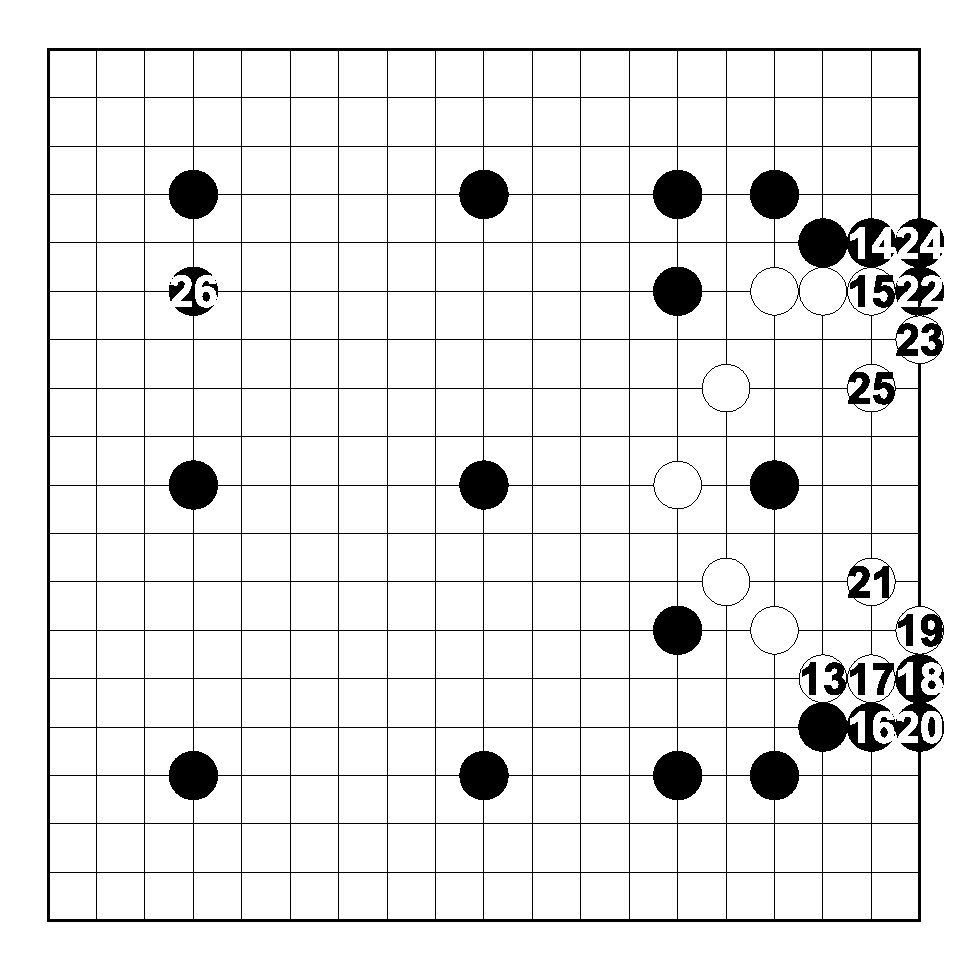
\includegraphics[width=.5\textwidth]{9 - Dia 6}
        \captionsetup{justification=centering}
        \caption*{\emph{Dia.\@~6}}
    \end{center}
    \vspace{-30pt}
\end{wrapfigure}

Ao avaliar essa posição, podemos perceber que Branco assegurou aproximadamente vinte e cinco pontos em um território já fortemente delimitado. Entretanto, os cantos Pretos são estimados em mais de quarenta pontos. Adicionalmente, Preto terminou em sente, então ele ainda pôde reforçar sua posição no canto superior esquerdo com 26. Esse movimento tornará uma invasão branca nessa região exponencialmente mais difícil.

\pagebreak

\section{Evitando a Estratégia Branca de Chapelação}

\begin{wrapfigure}{r}{60mm}
    \vspace{-27.5pt}
    \begin{center}
        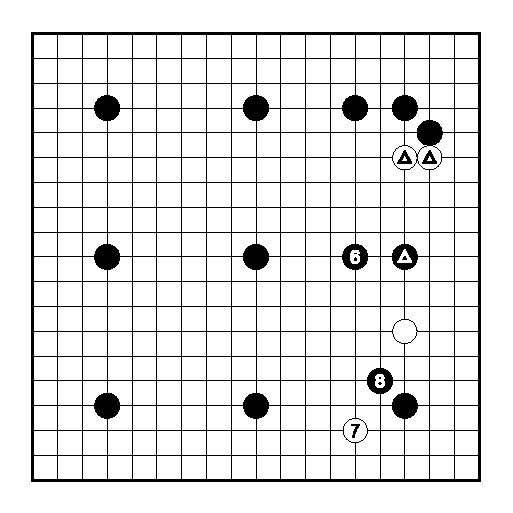
\includegraphics[width=.5\textwidth]{9 - Dia 7}
        \captionsetup{justification=centering}
        \caption*{\emph{Dia.\@~7}}
    \end{center}
    \vspace{-37.5pt}
\end{wrapfigure}

Ao invés de responder Branco 5 com 6 no \emph{Dia.\@~3}, uma jogada mais positiva é o pulo até 6 no \emph{Dia.\@~7}. Há duas razões por que esse é um bom movimento.

Primeiramente, Preto 6 cria uma barreira entre a pedra em 5 e a pedra branca marcada acima, assim mantendo os grupos separados. Branco agora está fragmentado em dois grupos sob ataque.

Em segundo lugar, Preto 6 se certifica de que a pedra marcada poderá se conectar à sua pedra no centro.

É esperado que Branco faça uma dupla-aproximação contra a pedra de compensação no canto inferior direito. Preto deveria então responder com o movimento diagonal em 8. Esse movimento segue o mesmo princípio de Preto 6: ele mantém as pedras brancas de 5 a 7 separadas e oferece acesso ao centro para a pedra 4-4, fazendo com que seja mais fácil conectá-la a seus aliados no exterior.

Há várias maneiras de Branco responder a Preto 8. Ele talvez ignore tal movimento e jogue em um lugar totalmente diferente; ele talvez, também, construa uma posição no lado inferior; ou ele talvez invada o canto como no \emph{Dia.\@~8} da próxima página.

\pagebreak

\section{Construindo Armações em Formato de Caixa}

\begin{wrapfigure}{r}{60mm}
    \vspace{-27.5pt}
    \begin{center}
        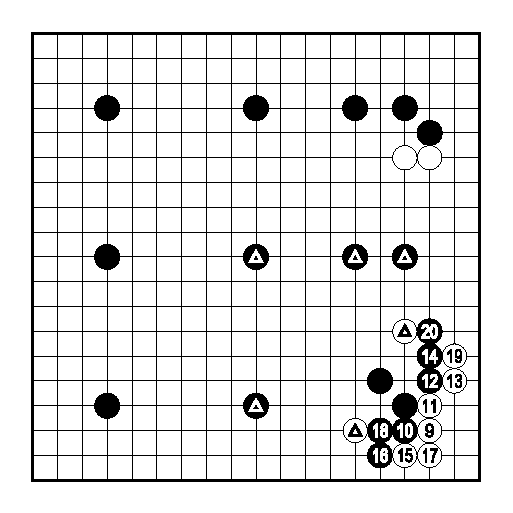
\includegraphics[width=.5\textwidth]{9 - Dia 8}
        \captionsetup{justification=centering}
        \caption*{\emph{Dia.\@~8}}
    \end{center}
    \vspace{-32.5pt}
\end{wrapfigure}

Branco geralmente responde Preto 8 invadindo o canto com 9 no \emph{Dia.\@~8}, mas isso não terá um bom resultado para ele. Preto bloqueia com 10, e Branco cria um grupo vivo no canto com os movimentos até 19. Porém, com 20, Preto consegue uma parede densa virada para o centro, constituindo uma armação de território em formato de caixa jundo com as pedras marcadas. Além disso, as duas pedras brancas marcadas são basicamente inúteis à sombra da parede preta.

\begin{wrapfigure}{l}{60mm}
    \vspace{-27.5pt}
    \begin{center}
        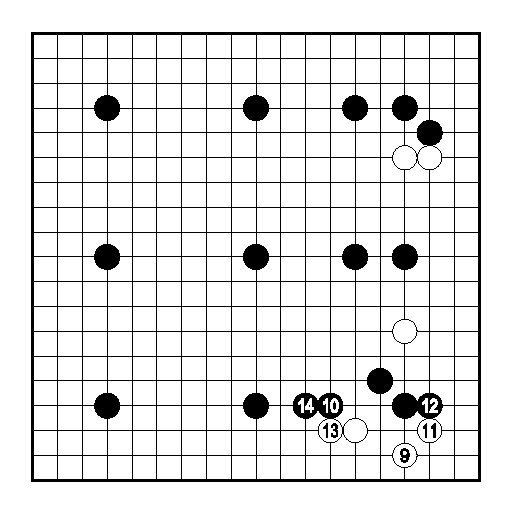
\includegraphics[width=.5\textwidth]{9 - Dia 9}
        \captionsetup{justification=centering}
        \caption*{\emph{Dia.\@~9}}
    \end{center}
    \vspace{-80pt}
\end{wrapfigure}

\bigskip

Branco talvez tente deslizar  para 9 no \emph{Dia.\@~9}. Novamente, Preto almeja o centro ao jogar 10. Branco cria um grupo vivo com 11 e 13, mas Preto mapeia uma grande armação de território em formato de caixa com 12 e 14. Com jogo claro e limpo, isso deveria gerar mais de 40 pontos garantidos de território para Preto.

\pagebreak

Branco poderia estender para 9, no \emph{Dia.\@~10}, esperando parar o avanço preto rumo à grande armação. Preto ancorará suas pedras no canto com 10. Se Branco pular para 11, Preto mantém Branco separado em dois. Branco terá muitas dificuldades vivendo com ambos os grupos.

\begin{figure}[h!]
    \centering
    \begin{subfigure}[t]{.5\textwidth}
        \centering
        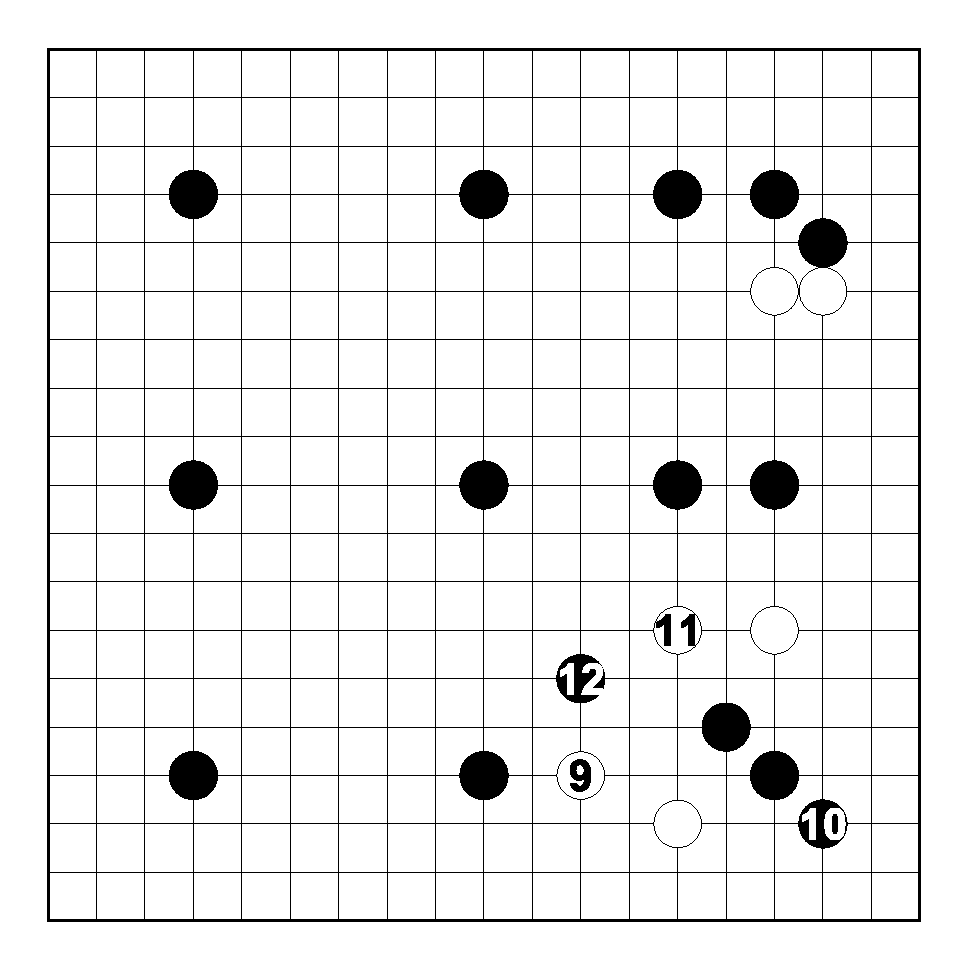
\includegraphics[width=1\textwidth]{9 - Dia 10}
        \captionsetup{justification=centering}
        \caption*{\emph{Dia.\@~10}}
    \end{subfigure}
\end{figure}

\pagebreak

\section{Expanda o Seu Território Atacando}

\begin{wrapfigure}{r}{60mm}
    \vspace{-27.5pt}
    \begin{center}
        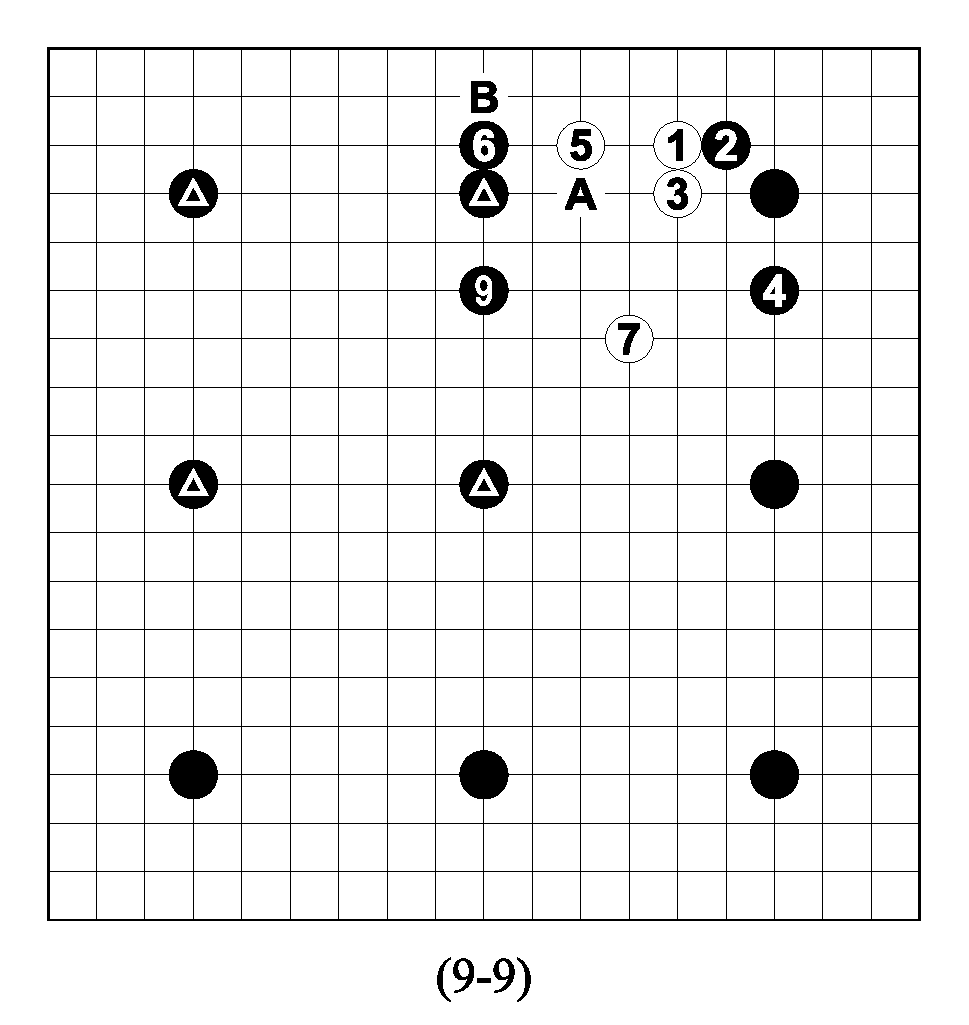
\includegraphics[width=.5\textwidth]{9 - Dia 11}
        \captionsetup{justification=centering}
        \caption*{\emph{Dia.\@~11}}
    \end{center}
    \vspace{-25pt}
\end{wrapfigure}

Depois da troca de 1 por Preto 4, Branco talvez tente criar uma base para suas pedras estendendo até 5 (ou \textbf{A}) em \emph{Dia.\@~11}. A resposta preta mais forte é fazer o ``pilar de ferro'' com 6. Essa jogada previne a base branca no contato em 6 ou o deslize em \textbf{B}. Esse pilar de ferro também reforça a formação de caixa delineada pelas pedras marcadas.

Branco não possui espaço para expansão no topo, então ele se expande ao centro. Preto mantém a pressão nas pedras brancas pulando a 8 e continuando a expandir e fortalecer sua armação no lado esquerdo.

\begin{wrapfigure}{l}{60mm}
    \vspace{-25pt}
    \begin{center}
        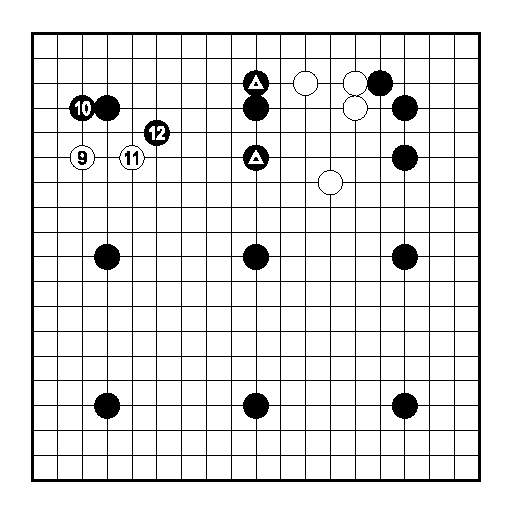
\includegraphics[width=.5\textwidth]{9 - Dia 12}
        \captionsetup{justification=centering}
        \caption*{\emph{Dia.\@~12}}
    \end{center}
    \vspace{-25pt}
\end{wrapfigure}

\bigskip

Já que Preto reforçou sua formação de caixa no canto superior esquerdo com as pedras marcadas, Branco estará em desvantagem se ali invadir. Portanto, ele talvez opte por jogar em uma parte do tabuleiro onde Preto possui menos pedras, esperando que qualquer posição que ele construa ali negue a influência preta da armação no canto superior esquerdo. No entanto, se ele tentar invadir essa área com 9 no \emph{Dia.\@~12}, Preto simplesmente enclausurará o canto com 10. Pular para Branco 11 é uma resposta razoável, mas Preto delimita o território no canto topo com 12. Jogando-se corretamente, Preto pode contar com pelo menos 25 pontos nessa região se tornando território seguro. No meio-tempo, Branco assegurou quase nenhum território e ele ainda possui duas pedras no lado esquerdo que precisam se estabilizar.

\begin{wrapfigure}{r}{60mm}
    \vspace{-27.5pt}
    \begin{center}
        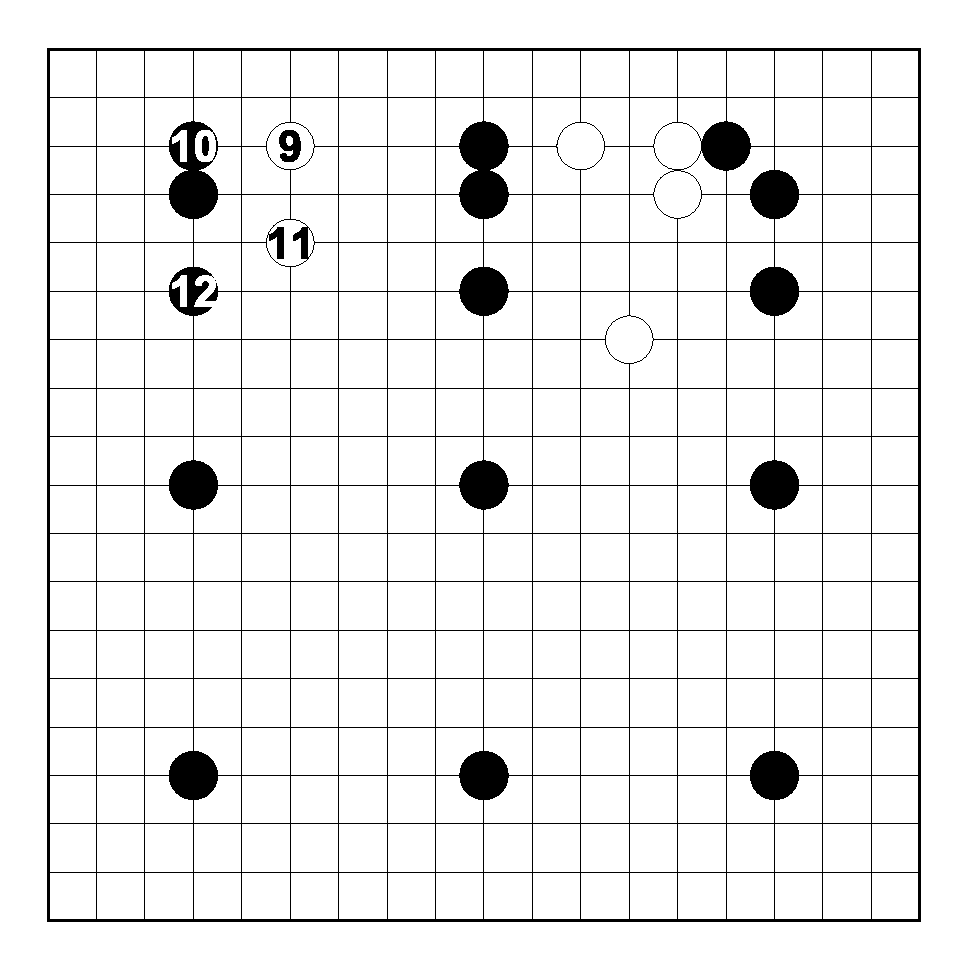
\includegraphics[width=.5\textwidth]{9 - Dia 13}
        \captionsetup{justification=centering}
        \caption*{\emph{Dia.\@~13}}
    \end{center}
    \vspace{-10pt}
\end{wrapfigure}

Se Branco se aproximar do outro lado com 9 no \emph{Dia.\@~13}, Preto irá novamente enclausurar o canto com 10, dessa maneira assegurando o território no lado esquerdo com 12, após o pulo branco até 11. Este resultado é ainda pior para Branco do que \emph{Dia.\@~12}, visto que suas pedras de 9 a 11 estão espremidas  entre duas posições fortes pretas. Será uma tarefa árdua se estabilizar com tal grupo branco.

\begin{wrapfigure}{l}{60mm}
    \vspace{-25pt}
    \begin{center}
        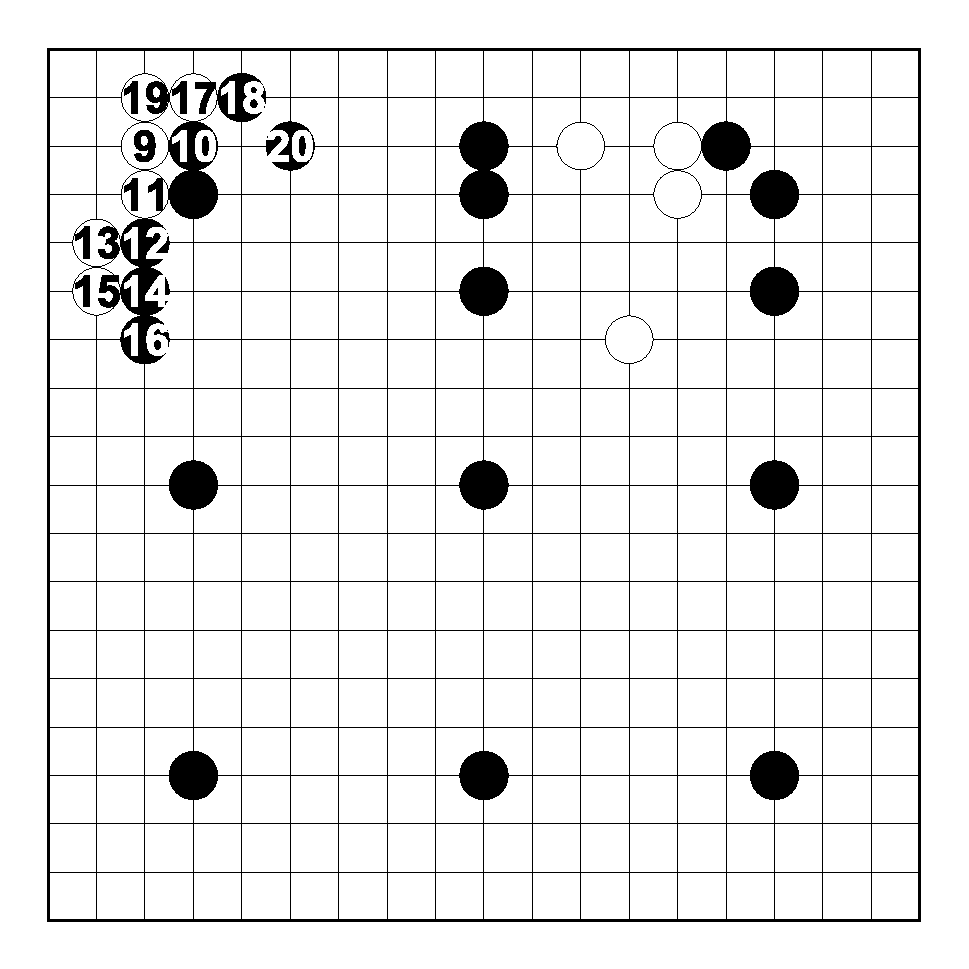
\includegraphics[width=.5\textwidth]{9 - Dia 14}
        \captionsetup{justification=centering}
        \caption*{\emph{Dia.\@~14}}
    \end{center}
    \vspace{-25pt}
\end{wrapfigure}

Por fim, Branco talvez invada diretamente o canto com 9 no \emph{Dia.\@~14}. Ele certamente pode criar um grupo vivo com quase dez pontos de território, mas à concessão de quase 30 pontos de potencial território, que muito provavelmente o será, com jogadas corretas.

\bigskip

Este capítulo é somente uma breve introdução à estratégia de compensação, em particular, a de nove pedras. Para uma discussão mais detalhada dessas posições, referenciam-se ao leitor \emph{Handicap Go Strategy and the Sanrensei Opening}~\cite{zeijst_bozulich_handicap_sanrensei}, disponível em forma impressa pela Kiseido (veja o \autoref{ap:pt} de catálogo de livros); ou, em sistemas iOS, o aplicativo SmartGo. Esse livro também é uma boa introdução a Go com compensação, assim como à abertura sanrensei, que é uma abertura de partidas em igualdade. Para um livro ainda mais detalhado sobre esse tópico, veja \emph{Handicap Go}~\cite{nagahara_bozulich_handicap_go}, também publicado pela Kiseido e disponível no aplicativo \href{apps.apple.com/us/app/smartgo-player/id314506629}{SmartGo}~\cite{smartgo}.